\documentclass[tikz,border=8pt]{standalone}
% Shared look for every TikZ diagram. Load with \input{../../tools/tikz-style.tex}
\usepackage[T1]{fontenc}
\usepackage{lmodern}
\renewcommand{\sfdefault}{lmr}  % diagrams use the same serif as the text
\usetikzlibrary{arrows.meta, positioning, shapes.geometric, calc, fit, backgrounds}
\definecolor{cblue}{HTML}{4C78A8}
\definecolor{corange}{HTML}{F58518}
\definecolor{cgreen}{HTML}{54A24B}
\definecolor{cred}{HTML}{E45756}
\definecolor{cpurple}{HTML}{B279A2}
\definecolor{cgrey}{HTML}{6B6B6B}
\tikzset{
  every picture/.style={font=\sffamily, line width=1.2pt},
  box/.style={draw=#1, fill=#1!12, rounded corners=4pt, align=center, inner sep=7pt, minimum height=1.1cm},
  box/.default=cgrey,
  arrow/.style={-{Stealth[length=3mm]}, draw=cgrey, line width=1.4pt},
  title/.style={font=\sffamily\bfseries\Large},
  note/.style={font=\sffamily\small, text=cgrey, align=center},
}
\AtBeginDocument{\hyphenpenalty=10000 \exhyphenpenalty=10000}

% The room of the Note: 7 m x 4 m, door in the top wall (3.0 to 4.2 m), a table (four-sided convex polygon), an
% L-shaped cabinet, a pink pole at (1, 3) and a green pole at (6, 0.8), and the robot at (2, 1) facing 30 degrees.
\begin{document}
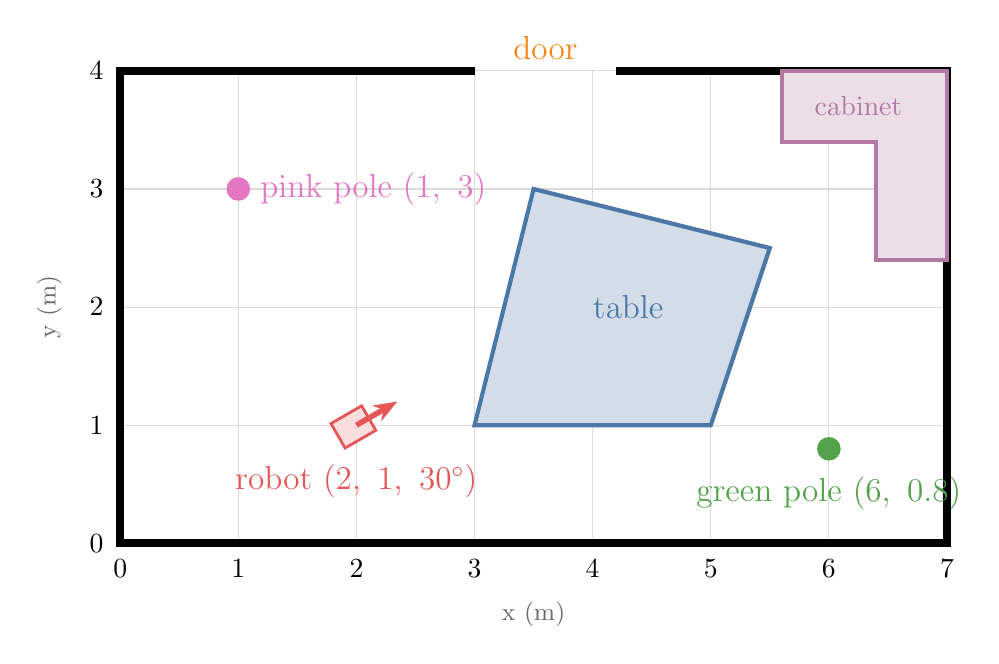
\begin{tikzpicture}[scale=1.5, every node/.append style={font=\large}]
  \definecolor{cpink}{HTML}{E377C2}
  \draw[cgrey!25, line width=0.4pt] (0,0) grid (7,4);
  \draw[black, line width=3pt] (3.0,4) -- (0,4) -- (0,0) -- (7,0) -- (7,4) -- (4.2,4);
  \node[corange, above] at (3.6,4.0) {door};
  \filldraw[cblue!25, draw=cblue, line width=1.5pt] (3,1) -- (5,1) -- (5.5,2.5) -- (3.5,3) -- cycle;
  \node[cblue] at (4.3,2.0) {table};
  \filldraw[cpurple!25, draw=cpurple, line width=1.5pt] (5.6,4) -- (5.6,3.4) -- (6.4,3.4) -- (6.4,2.4) -- (7,2.4) -- (7,4) -- cycle;
  \node[cpurple, align=center, font=\normalsize] at (6.25,3.7) {cabinet};
  \fill[cpink] (1,3) circle (0.1); \node[cpink, right=4pt] at (1,3) {pink pole $(1,\ 3)$};
  \fill[cgreen] (6,0.8) circle (0.1); \node[cgreen, below=4pt] at (6,0.75) {green pole $(6,\ 0.8)$};
  \begin{scope}[shift={(2,1)}, rotate=30]
    \draw[cred, fill=cred!20, line width=1pt] (-0.18,-0.12) rectangle (0.12,0.12);
    \draw[-{Stealth[length=3mm]}, cred, line width=2pt] (0,0) -- (0.4,0);
  \end{scope}
  \node[cred, below=6pt] at (2,0.9) {robot $(2,\ 1,\ 30^\circ)$};
  \foreach \t in {0,...,7} \node[below, font=\normalsize] at (\t,-0.05) {\t};
  \foreach \t in {0,...,4} \node[left, font=\normalsize] at (-0.05,\t) {\t};
  \node[note] at (3.5,-0.6) {x (m)}; \node[note, rotate=90] at (-0.6,2) {y (m)};
\end{tikzpicture}
\end{document}
